\section{\normalsize  Второе начало термодинамики. Неравенство и равенство Клаузиуса. Энтропия. Закон возрастания энтропии. Энтропия идеального газа.}
\paragraph{Второе начало термодинамики.} \textbf{Формулировка Клаузиуса:} невозможен круговой процесс, единственным результатом которого был бы переход тепла от более холодного тела к более нагретому.\\
\textbf{Формулировка Томпсона:} невозможен круговой процесс, единственным результатом которого было бы производство работы за счет охлаждения теплового резервуара. Формулировки Клаузиуса и Томпсона эквивалентны. \\
\textbf{Формулировка Планка:} невозможно построить периодически действующую машину, единственным результатом которой было бы поднятие груза за счёт охлаждения теплового резервуара.
\paragraph{Неравенство Клаузиуса.} Имеем $n$ тепловых резервуаров $R_1,\ldots,R_n$ достаточно больших, чтобы в процесса теплообмена $T_1,\ldots,T_n\simeq const.$\\
Таким образом система I совершила круговой процесс, заимствова $Q_1$ у $R_1,\ldots,Q_n$ у $R_n$, совершив $A=Q_1+\ldots+Q_n$\\
После совершения цикла возьмем $R_0$ с $T_0$, также достаточно большой и $n$ машин Карно $K_1,\ldots,K_n$, включив их как показано на рисунке. Синхронность их работы и количество не важно.\\
\begin{minipage}{55 mm}
	\begin{figure}[H]
		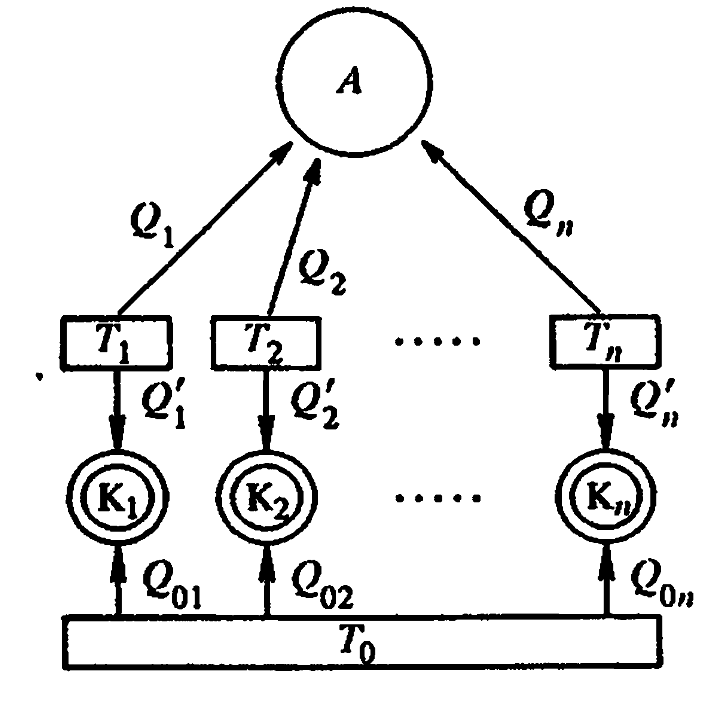
\includegraphics[width=50mm]{ris.png}
	\end{figure}
\end{minipage}
\begin{minipage}{115mm}
	Для i-ой машины за 1 цикл: $1+\dfrac{Q_i'}{Q_{oi}}=1-\dfrac{T_i}{T_o} \Leftrightarrow\dfrac{Q_{oi}}{T_o}+\dfrac{Q_i'}{T_i}=0$.\\
	Суммируя по i: $Q_o=\sum_iQ_{oi}=-T_o\sum_i\dfrac{Q_i'}{T_i}$\\
	$Q_o$ --- общее количество теплоты, отданное $R_o$. Объединим все $n$ циклов машин Карно с циклом I в один большой: $R_o$ отдал $Q_o$; $R_1$ отдал $Q_1+Q_1';\ldots\;R_n$ отдал $Q_n+Q_n'$. Совершена работа $A=Q_o+(Q_1+Q_1')+\ldots(Q_n+Q_n')$. В силу больших размеров $R_1,\ldots,R_n$ выберем в согласии с постулатом Томпсона--Планка $Q_1',\ldots,Q_n'$ так, что \\
	$Q_i'+Q_i=0,\,i=\overline{1,n}\then$ все тепловые резервуары вернутся в исходное состояние, а $R_o$ отдаст $Q_o=T_o\sum_{i=1}^{n}\dfrac{Q_i}{T_i}$\\
	Таким образом совершается круговой процесс, за который отдано $Q_o$ и совершена работа $A=Q_o$. Других изменений не произошло. Тогда $A\leqslant0$ из постулата Томпсона--Планка, значит $Q_o\leqslant0$ \\
\end{minipage}
Переходя к пределу бесконечно большого числа тепловых резервуаров $R_1,\ldots$, обменивающихся бесконечно малыми порциями тепла с I и $R_o$ получаем:
$$\oint\dfrac{\delta Q}{T}\leqslant0\text{ --- \textbf{неравенство Клаузиуса}}$$
$T$ --- температура теплового резервуара, с которым система в данным момент обменивается теплом. В квазистатическом цикле под $T$ можно понимать температуру окружающей среды, так как обе температуры одинаковы.\\
Квазистатический процесс обратим, следовательно справедливо $\oint\dfrac{\delta Q'}{T}\leqslant0$, где $\delta Q'$ --- элементарное количество теплоты, получаемое системой на отдельных участках процесса. Так как процесс идет через те же состояния, то $\delta Q=-\delta Q'\then\oint\dfrac{\delta Q}{T}\geqslant$. А такое соотношение верно только тогда, когда $$\oint_\text{квазист.}\dfrac{\delta Q}{T}=0\text{ --- \textbf{равенство Клаузиуса}}$$
\paragraph{Энтропия.} Рассмотрим 2 способа перехода из 1 в 2, каждый из которых --- квазистатический процесс. Объединим их в круговой 1\RomanNumeralCaps{1}2\RomanNumeralCaps{2}1 и применим равенство Клаузиуса.
$$\int_{1\RomanNumeralCaps{1}2}\dfrac{\delta Q}{T} + \int_{2\RomanNumeralCaps{2}1}\dfrac{\delta Q}{T}=0\Leftrightarrow\int_{1\RomanNumeralCaps{1}2}\dfrac{\delta Q}{T}=\int_{2\RomanNumeralCaps{2}1}\dfrac{\delta Q}{T}\text{ --- приведённое количество теплоты.}$$
Таким образом приведённое количество теплоты, полученное системой при любом квазистатическом круговом процессе равно нулю \textbf{или} приведённое количество теплоты, полученное системой в квазистатическом процессе, не зависит от пути перехода, а определяется лишь начальным и конечным состояниями.\\
Отсюда: \textbf{энтропия} --- функция состояния системы, определённая с точностью до константы.
$$\Delta S \equiv \int_{1\rightarrow2}\dfrac{\delta Q}{T},\;\;dS=\left(\dfrac{\delta Q}{T}\right)_\text{кваз.}$$
\paragraph{Энтропия идеального газа.}
\textbf{Для идеального газа:} $$\delta Q=C_VdT+PdV=C_V(T)dT+R\dfrac{dV}{V}T\Leftrightarrow dS=\dfrac{\delta Q}{T}=C_V(T)\dfrac{dT}{T}+R\dfrac{dV}{V}$$
$$S=\int C_V(T)\dfrac{dT}{T}+R\int \dfrac{dV}{V}$$
Если $C_V$ не зависит от $T$, то $S=\nu(C_v\ln(T)+R\ln\left(\dfrac{V}{\nu}\right)+const)$. Всякий адиабатический процесс с $\delta Q=0\then dS=0\then S=const$.\\
\paragraph{Закон возрастания энтропии.} Энтропия адиабатически изолированной системы не может убывать, она либо растёт, либо постоянна. \\Система может переходить из 1 в 2 необратимо по \RomanNumeralCaps{1}. Вернём её квазистатически по какому-либо \RomanNumeralCaps{2}. Тогда
$\oint\dfrac{\delta Q}{T}=\int_\RomanNumeralCaps{1}\dfrac{\delta Q}{T}+\int_{\RomanNumeralCaps{2}}\dfrac{\delta Q}{T}\leqslant0$.
Так как $\int_{\RomanNumeralCaps{2}}\dfrac{\delta Q}{T}=S_1-S_2\then S_2-S_1\geqslant\int_{1\rightarrow2}\dfrac{\delta Q}{T}$. Если система адиабатически изолирована, то $\delta Q=0\then S_2\geqslant S_1$.
